\documentclass{minimal}
\usepackage{pgfplots}
\usepackage{pgfplotstable}
\pgfplotsset{compat=newest}

\begin{document}

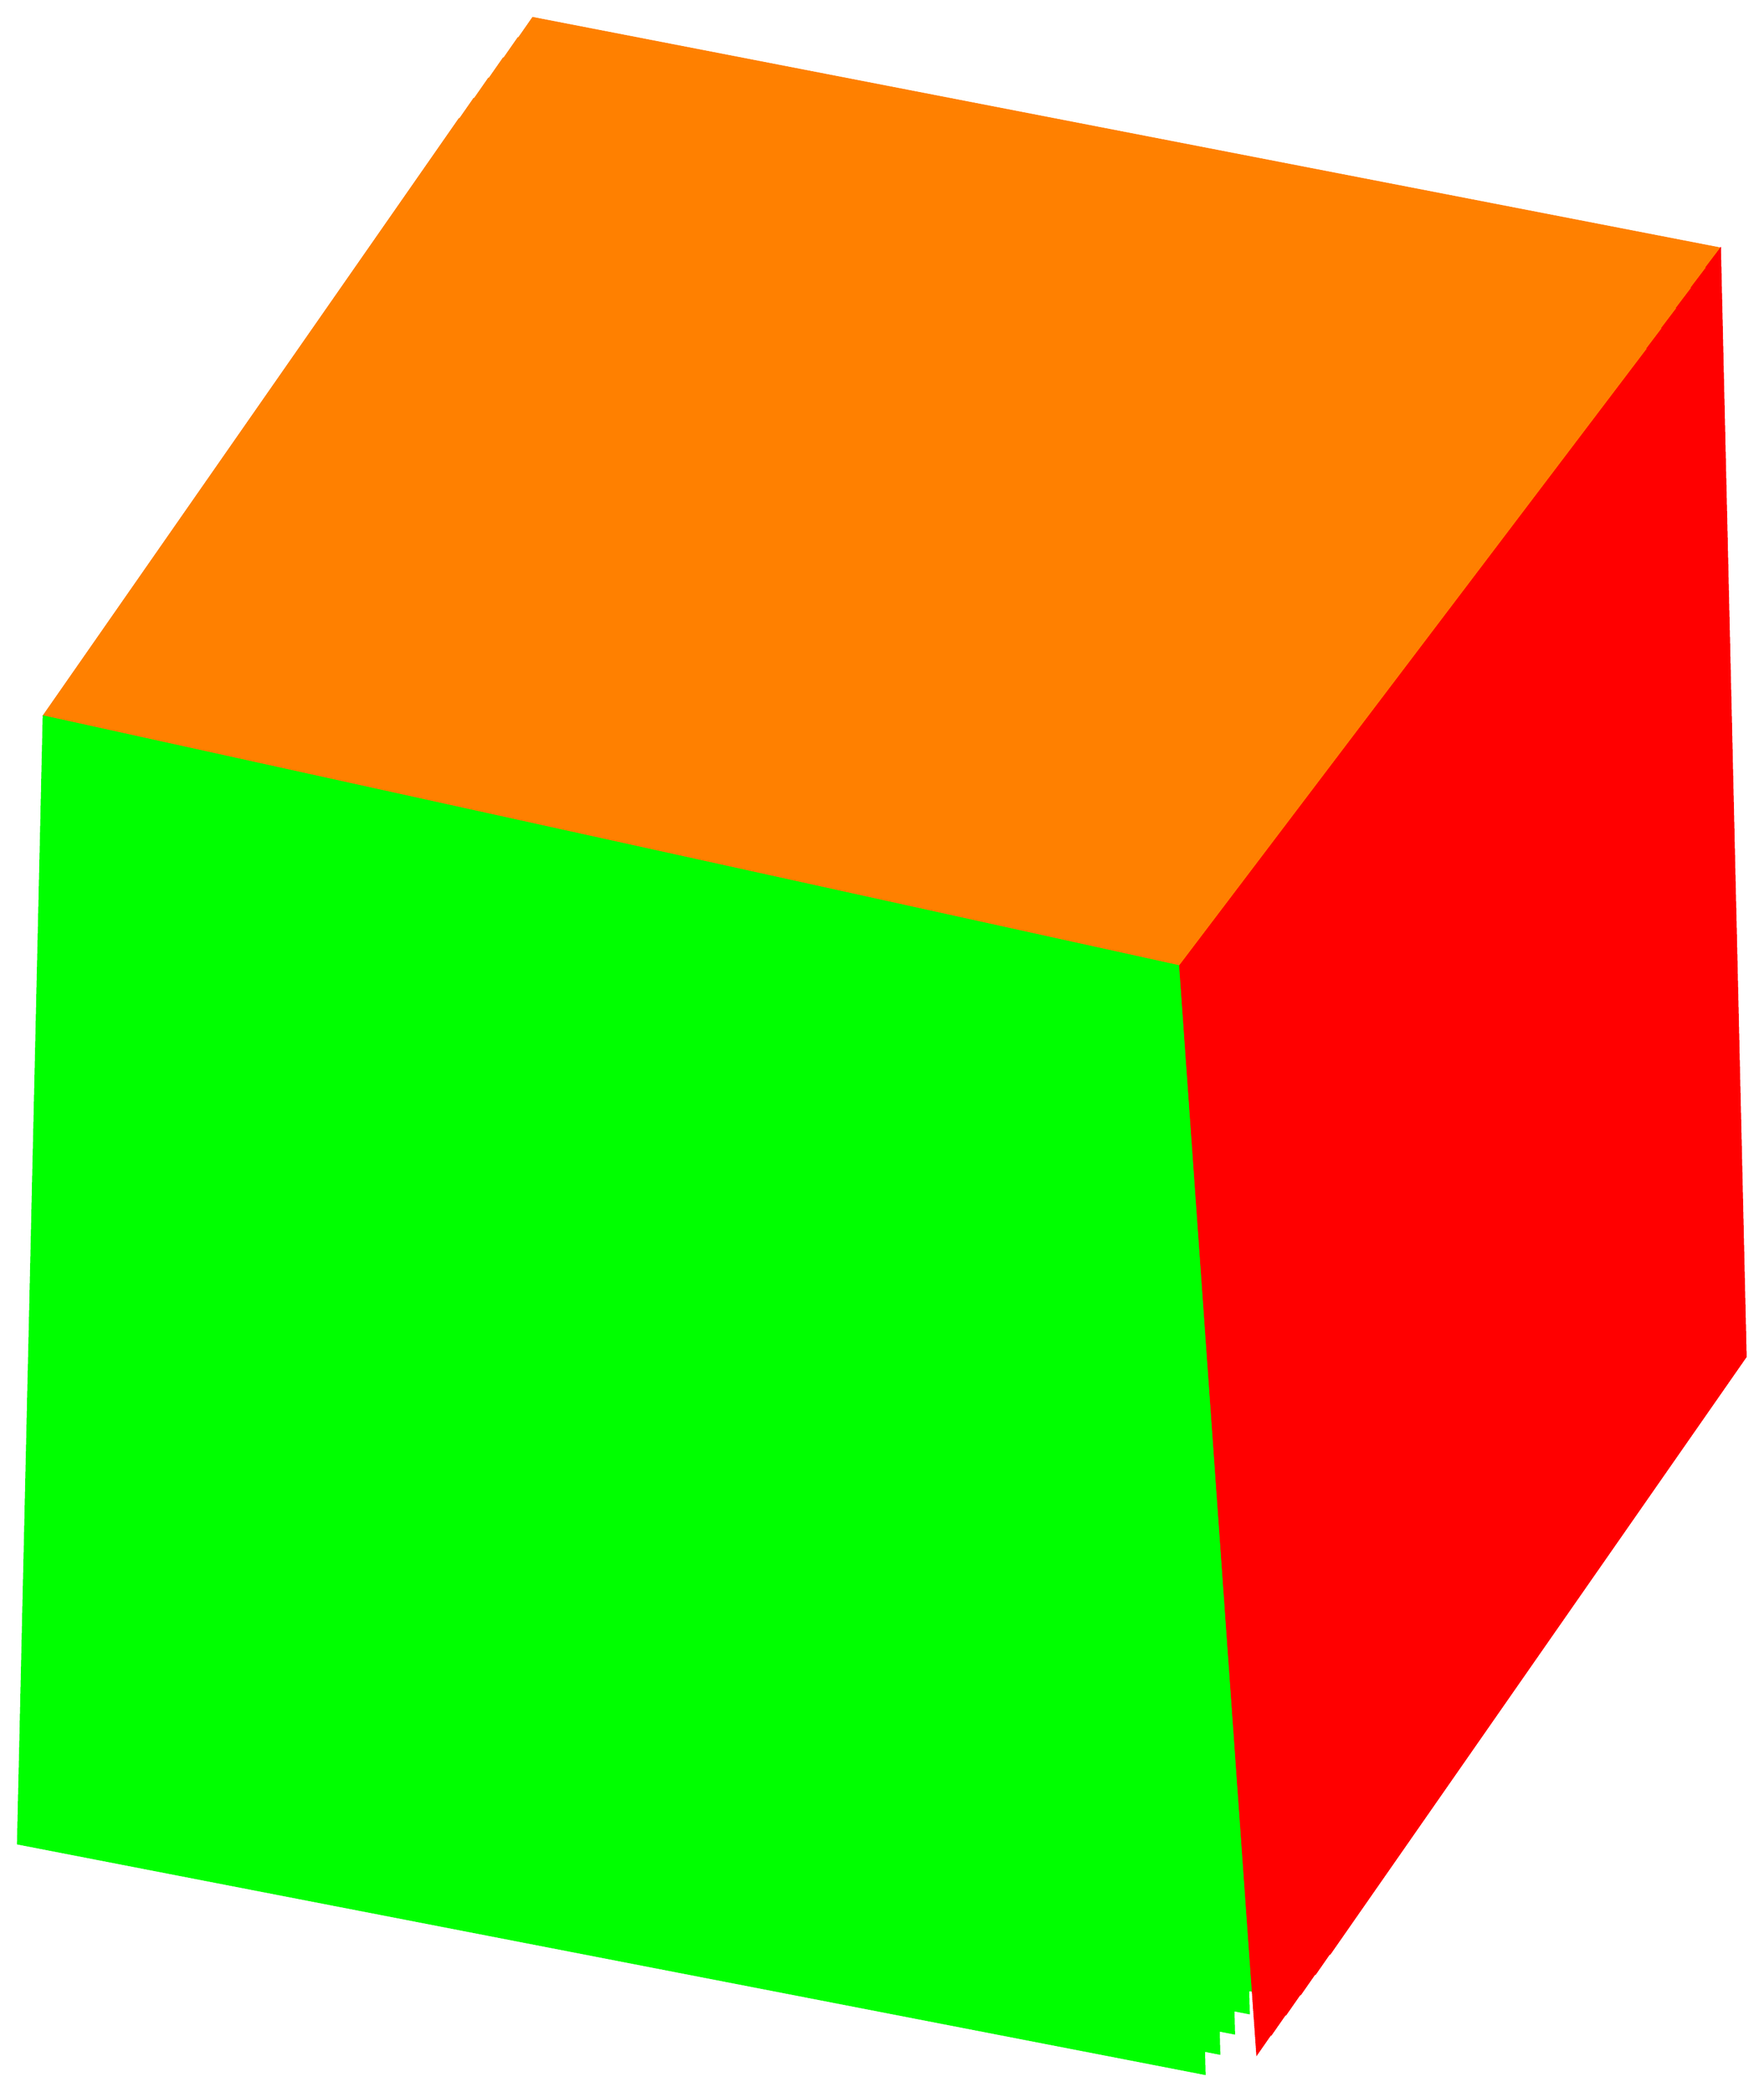
\begin{tikzpicture}

\pgfmathsetmacro{\cubex}{30}
\pgfmathsetmacro{\cubey}{30}
\pgfmathsetmacro{\cubez}{30}

\begin{axis}[view={110}{30},axis equal,
    xmin = -1,
    ymin = -1,
    xmax = 5,
    ymax = 1,
    zmin = -1,
    zmax = 1]
\definecolor{bouteillo}{RGB}{255,0,0}


\pgfdeclareplotmark{realcube}{
%\draw[fill] (0,0,0) -- ++(-100,0,0) -- ++(0,-100,0) -- ++(100,0,0) -- cycle;
%\draw[fill] (0,0,0) -- ++(0,0,-100) -- ++(0,-100,0) -- ++(0,0,100) -- cycle;
%\draw[fill] (0,0,0) -- ++(-100,0,0) -- ++(0,0,-100) -- ++(100,0,0) -- cycle;
%\fill [orange] (0,0,0) -- ++(-\cubex,0,0) -- ++(0,-\cubey,0) -- ++(\cubex,0,0) -- cycle;
%\fill[ green] (0,0,0) -- ++(0,0,-2*\cubez) -- ++(0,-\cubey,0) -- ++(0,0,2*\cubez) -- cycle;
%\fill [purple] (0,0,0) -- ++(-\cubex,0,0) -- ++(0,0,-2*\cubez) -- ++(\cubex,0,0) -- cycle;
\fill [orange] (\cubex/2,\cubey/2,\cubez) -- ++(-\cubex,0,0) -- ++(0,-\cubey,0) -- ++(\cubex,0,0) -- cycle;
\fill [green] (\cubex/2,\cubey/2,\cubez) -- ++(0,0,-\cubez) -- ++(0,-\cubey,0) -- ++(0,0,\cubez) -- cycle;
\fill [bouteillo] (\cubex/2,\cubey/2,\cubez) -- ++(-\cubex,0,0) -- ++(0,0,-\cubez) -- ++(\cubex,0,0) -- cycle;
    }

\foreach \iter in {0,1,...,5} {

\addplot3[scatter,mark=realcube,red] coordinates {%
    %(2,2,0) (2,2,1) (2,2,2) (1,2,0) (1,2,1) (1,2,2) (0,2,0) (0,2,1) (0,2,2) 
    %(2,1,0) (2,1,1) (2,1,2) (1,1,0) (1,1,1) (1,1,2) (0,1,0) (0,1,1) (0,1,2) 
    %(2,0,0) (2,0,1) (2,0,2) (1,0,0) (1,0,1) (1,0,2) (0,0,0) (0,0,1) (0,0,2) 
    
    %(0,0,0) (0,0,1) (0,0,2) (1,0,0) (1,0,1) (1,0,2) (2,0,0) (2,0,1) (2,0,2) 
    %(0,1,0) (0,1,1) (0,1,2) (1,1,0) (1,1,1) (1,1,2) (2,1,0) (2,1,1) (2,1,2) 
    %(0,2,0) (0,2,1) (0,2,2) (1,2,0) (1,2,1) (1,2,2) (2,2,0) (2,2,1) (2,2,2)  
    (\iter,0,0) %(1,0,0) (2,0,0) %(0,1,0) (1,1,0) (2,1,0) (0,2,0) (1,2,0) (2,2,0)
    %(0,0,1) (1,0,1) (2,0,1) (0,1,1) (1,1,1) (2,1,1) (0,2,1) (1,2,1) (2,2,1)
    %(0,0,2) (1,0,2) (2,0,2) (0,1,2) (1,1,2) (2,1,2) (0,2,2) (1,2,2) (2,2,2) 
    } ;
    }
\end{axis}
\end{tikzpicture}

\end{document}